\chapter{Evaluation}
\label{chap:Evaluation}

\section{Contexte}
Dans une tâche d'object detection, nous utilisons le score IoU qui signifie Intersection over Union.
C'est un score qui compare les bounding boxes prédites par le modèle avec les bounding boxes réels (ground-truth).
Une tâche d'object detection comprend deux sous-problèmes: la classification et la localisation.
Ainsi nous avons plusieurs métriques pour analyser la performance d'un modèle. IoU se concentre sur 
la localisation des bounding box prédites tandis que la métrique mAP (mean Average Precision) 
se concentre sur la classification.
\begin{figure}[bh!]
    \centering
    \scalebox{0.5}[0.5]{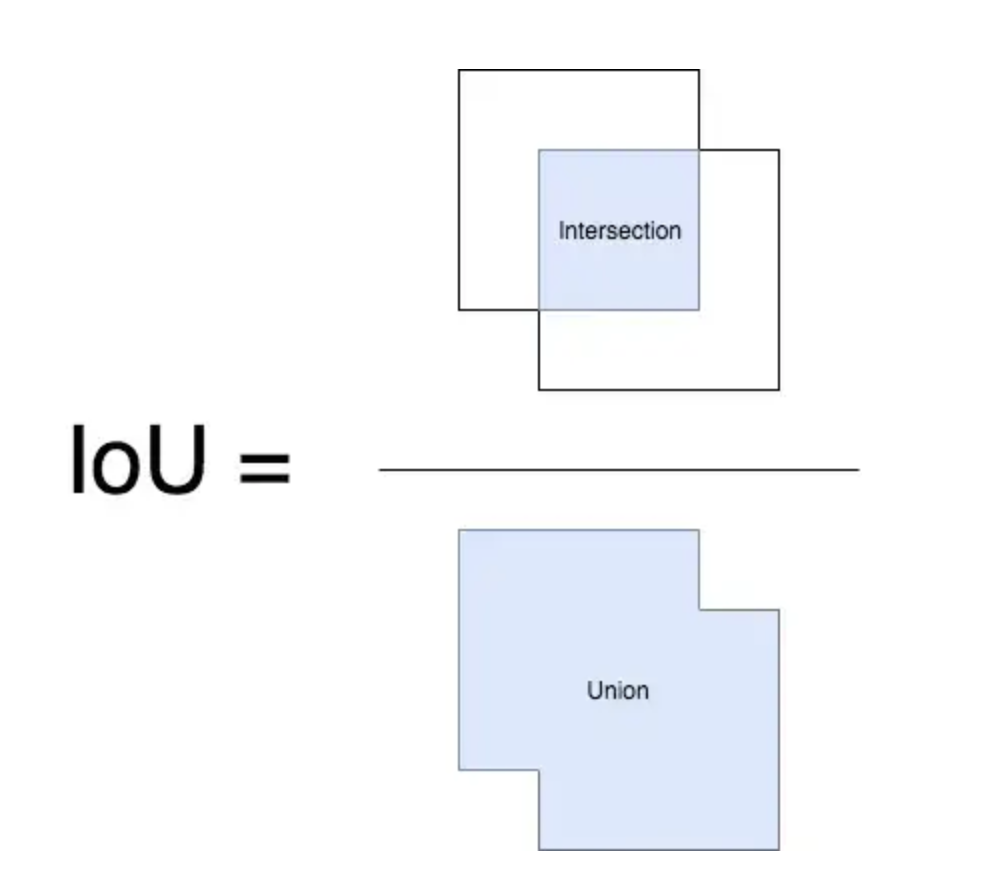
\includegraphics[width=\textwidth]{images/iou.png}}
    \caption{Intersection over Union}
    \label{fig:iou}
\end{figure}
Un score IoU de 1 signifie que la bounding box prédite est parfaitement superposée sur la bounding box réel, tandis qu'un score de 0 signifie qu'il n'y a pas d'air en commun. Idéalement on espère donc avoir un score IoU de 1 pour toutes nos bounding boxes
% -- Joris:


\section{Lecture d'un benchmark COCO}
Un benchmark COCO peut être affiché dans la console comme présenté dans l'image \ref{fig:eval_coco_benchmark}. Ce benchmark est réalisé en suivant l'API COCO\footnote[1]{\url{cocodataset.org/\#detection-eval}}. Il présente deux métrics la précision ($\displaystyle{\frac{TP}{TP+FP} }$) et le rappel ($\displaystyle{ \frac{TP}{TP+FN}}$).
\begin{figure}[h!]
    \centering
    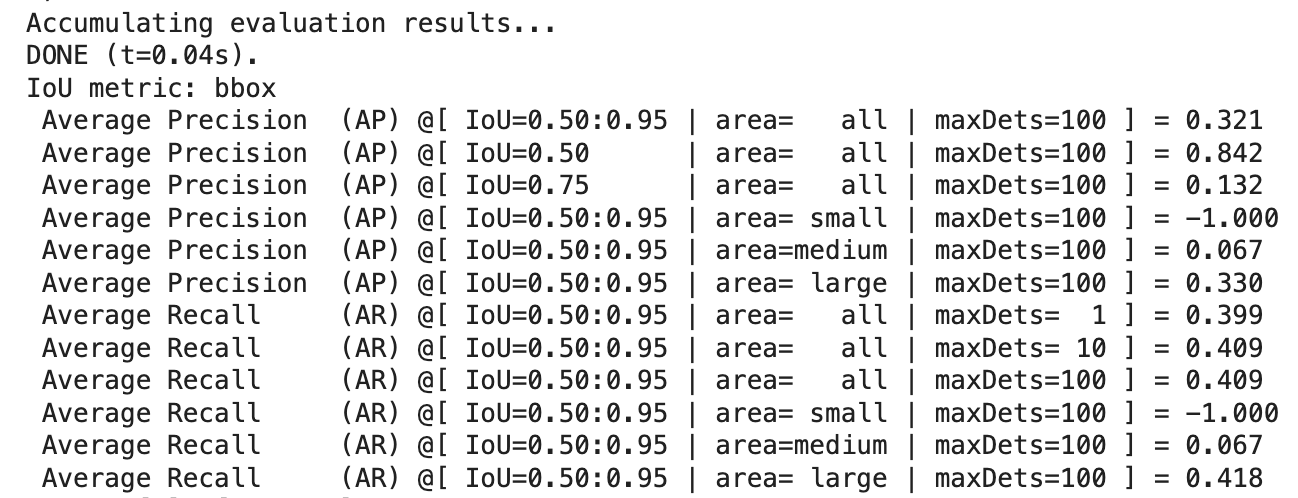
\includegraphics[width=\textwidth]{images/eval_coco_benchmark_white.png}
    \caption{Exemple de benchmark COCO dans la console}
    \label{fig:eval_coco_benchmark}
\end{figure}
La précision moyenne, (AP-Average Precision) présente dans les résultats COCO est calculée sur toutes les catégories, elle correspond traditionnellement au mean Average Precision (mAP).
Les résultats sont divisé en 4 catégories qui dépendent du score IoU ou de l'air de la bounding box prédite.
\begin{itemize}
    \item Les trois premières lignes sont l'AP en considérant différents seuil d'IoU pour sélectionner les boudings boxes à évaluer.
    \item Les trois suivantes sont l'AP en considérant des surfaces de tailles différentes pour sélectionner les boudings boxes à évaluer
    \item Les trois suivantes sont le Rappel Moyens (AR) en considérant plusieurs IoU pour sélectionner les boudings boxes à évaluer.
    \item Les trois suivantes sont l'AR en considérant des surfaces de tailles différentes pour sélectionner les boudings boxes à évaluer.
\end{itemize}
Selon la documentation, la première ligne est la plus importante. A la place de considérer les bounding boxes qui ont un IoU plus grand que le seuil, il est calculé sur cette ligne la moyenne des mAP des bounding boxes selon 10 seuils différents (de 0.5 à 0.95 par pas de 0.05).
%https://github.com/facebookresearch/detectron2/blob/main/MODEL_ZOO.md
Il faut noter que s'il n'existe pas de bounding boxes répondant aux critères, un score de \verb|-1| est affiché. On observe donc qu'il n'existe pas de bounding box de petite taille (32x32 pixels) puisque l'AP ainsi que l'AR où l'air est petite vaut \verb|-1|.
\paragraph{}
Avec Detectron2, un benchmark COCO est fait après chaque époch. C'est à dire lorsque le modèle à vu une fois le dataset en entier. Ce benchmark est effectué sur une fold du set d'entrainement appelé validation. Cependant, afin de véritablement tester les résutlats, nous avons aussi effectué un benchmark COCO sur un set de test d'images jamais vues par le modèle. 
Detectron2 sauvegarde les résultats dans un fichier json, ce fichier peut être lu par un widget TensorBoard afin de monitorer l'entrainement.
Les résultats peuvent aussi être visualisé de manière résumée, par défaut ce n'est pas fait durant l'entrainement uniquement lors d'un benchmark COCO complet. Le résumé s'affiche comme dans l'image \ref{fig:eval_coco_benchmark_resume} 
\begin{figure}
    \centering
    \scalebox{0.5}[0.5]{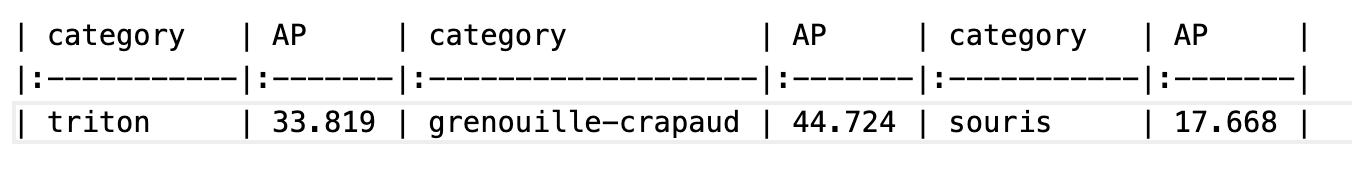
\includegraphics[width=\textwidth]{images/eval_coco_benchmark_resume.png}}
    \caption{Résumé COCO de FASTER RCNN}
    \label{fig:eval_coco_benchmark_resume}
\end{figure}
On voit très facilement que les AP sont désormais calculés par classes sans distinction de IoU. 


\section{Tensorboard de faster RCNN }\label{anal:train_rcnn}
Les widgets tensorboard permettent durant tous les entrainments d'avoir un aperçu des différentes métriques enregistrées nous pouvons donc savoir quand arrêter l'entrainement pour avoir la meilleur performance selon une métrique, cela permet aussi de ne pas overfit. Nous avons pris quelques captures d'écrans affichées dans les figures \ref{fig:tensorboard_overview} et \ref{fig:tensorboard_metric}
\begin{figure}[h!]
    \centering
    \begin{subfigure}[t]{0.49\textwidth}
        \centering
        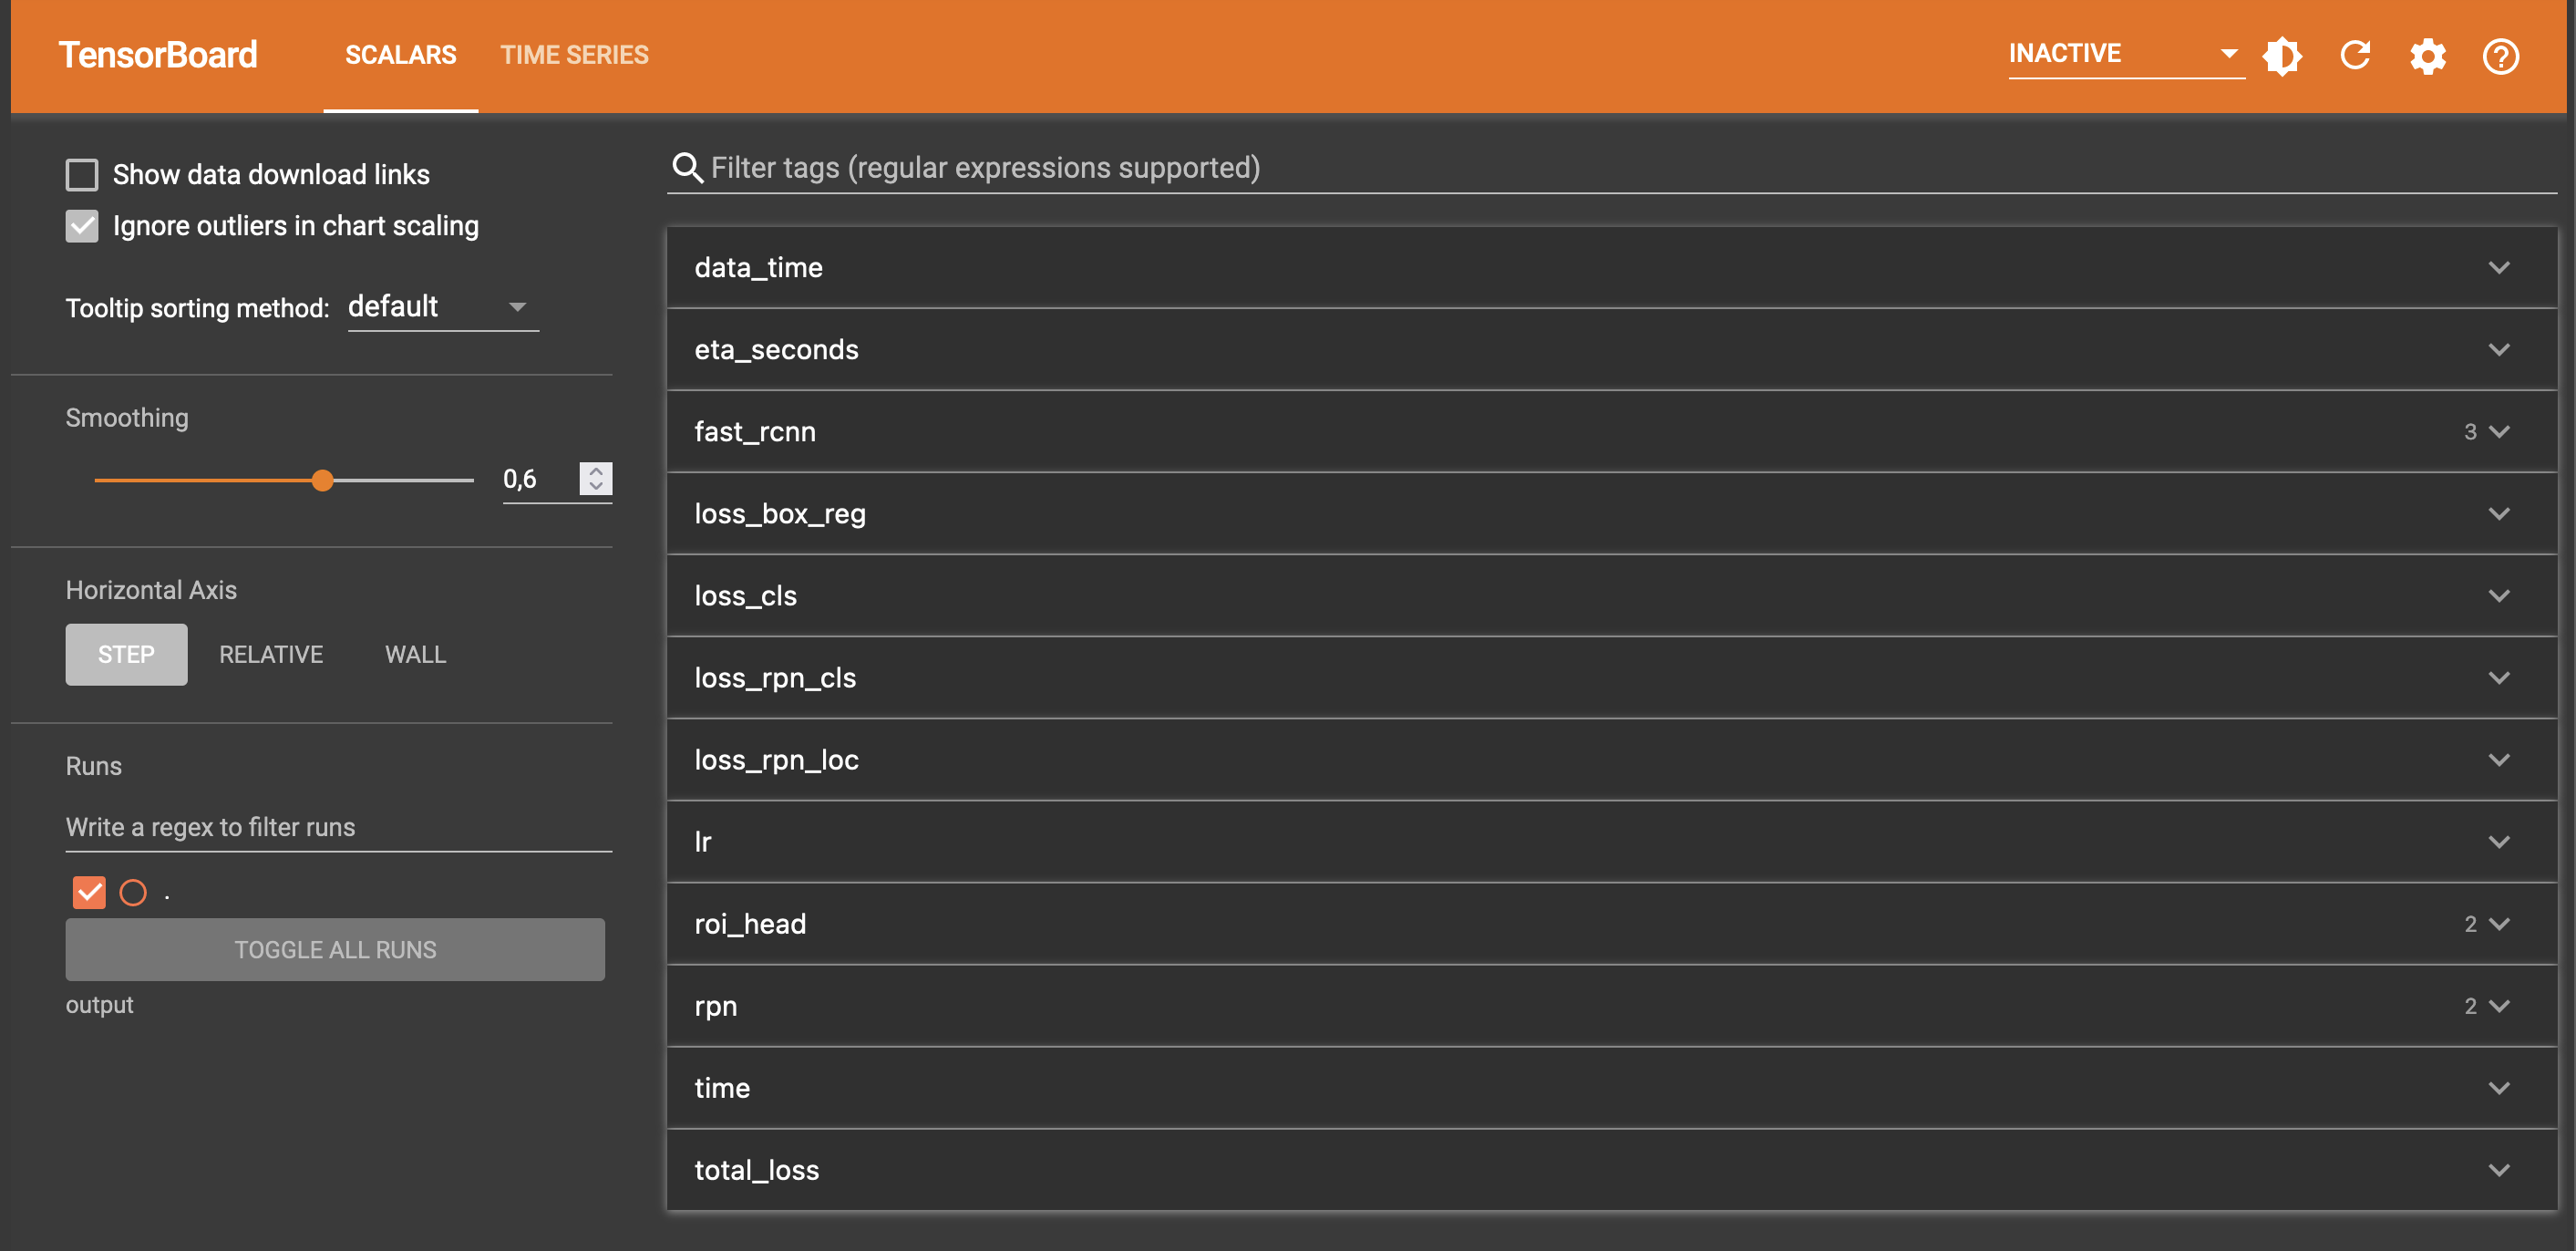
\includegraphics[width=\textwidth]{images/tensorboard_large.png}
        \caption{Aperçu du widget Tensorboard}
        \label{fig:tensorboard_overview}
    \end{subfigure}
    \begin{subfigure}[t]{0.49\textwidth}
        \centering
        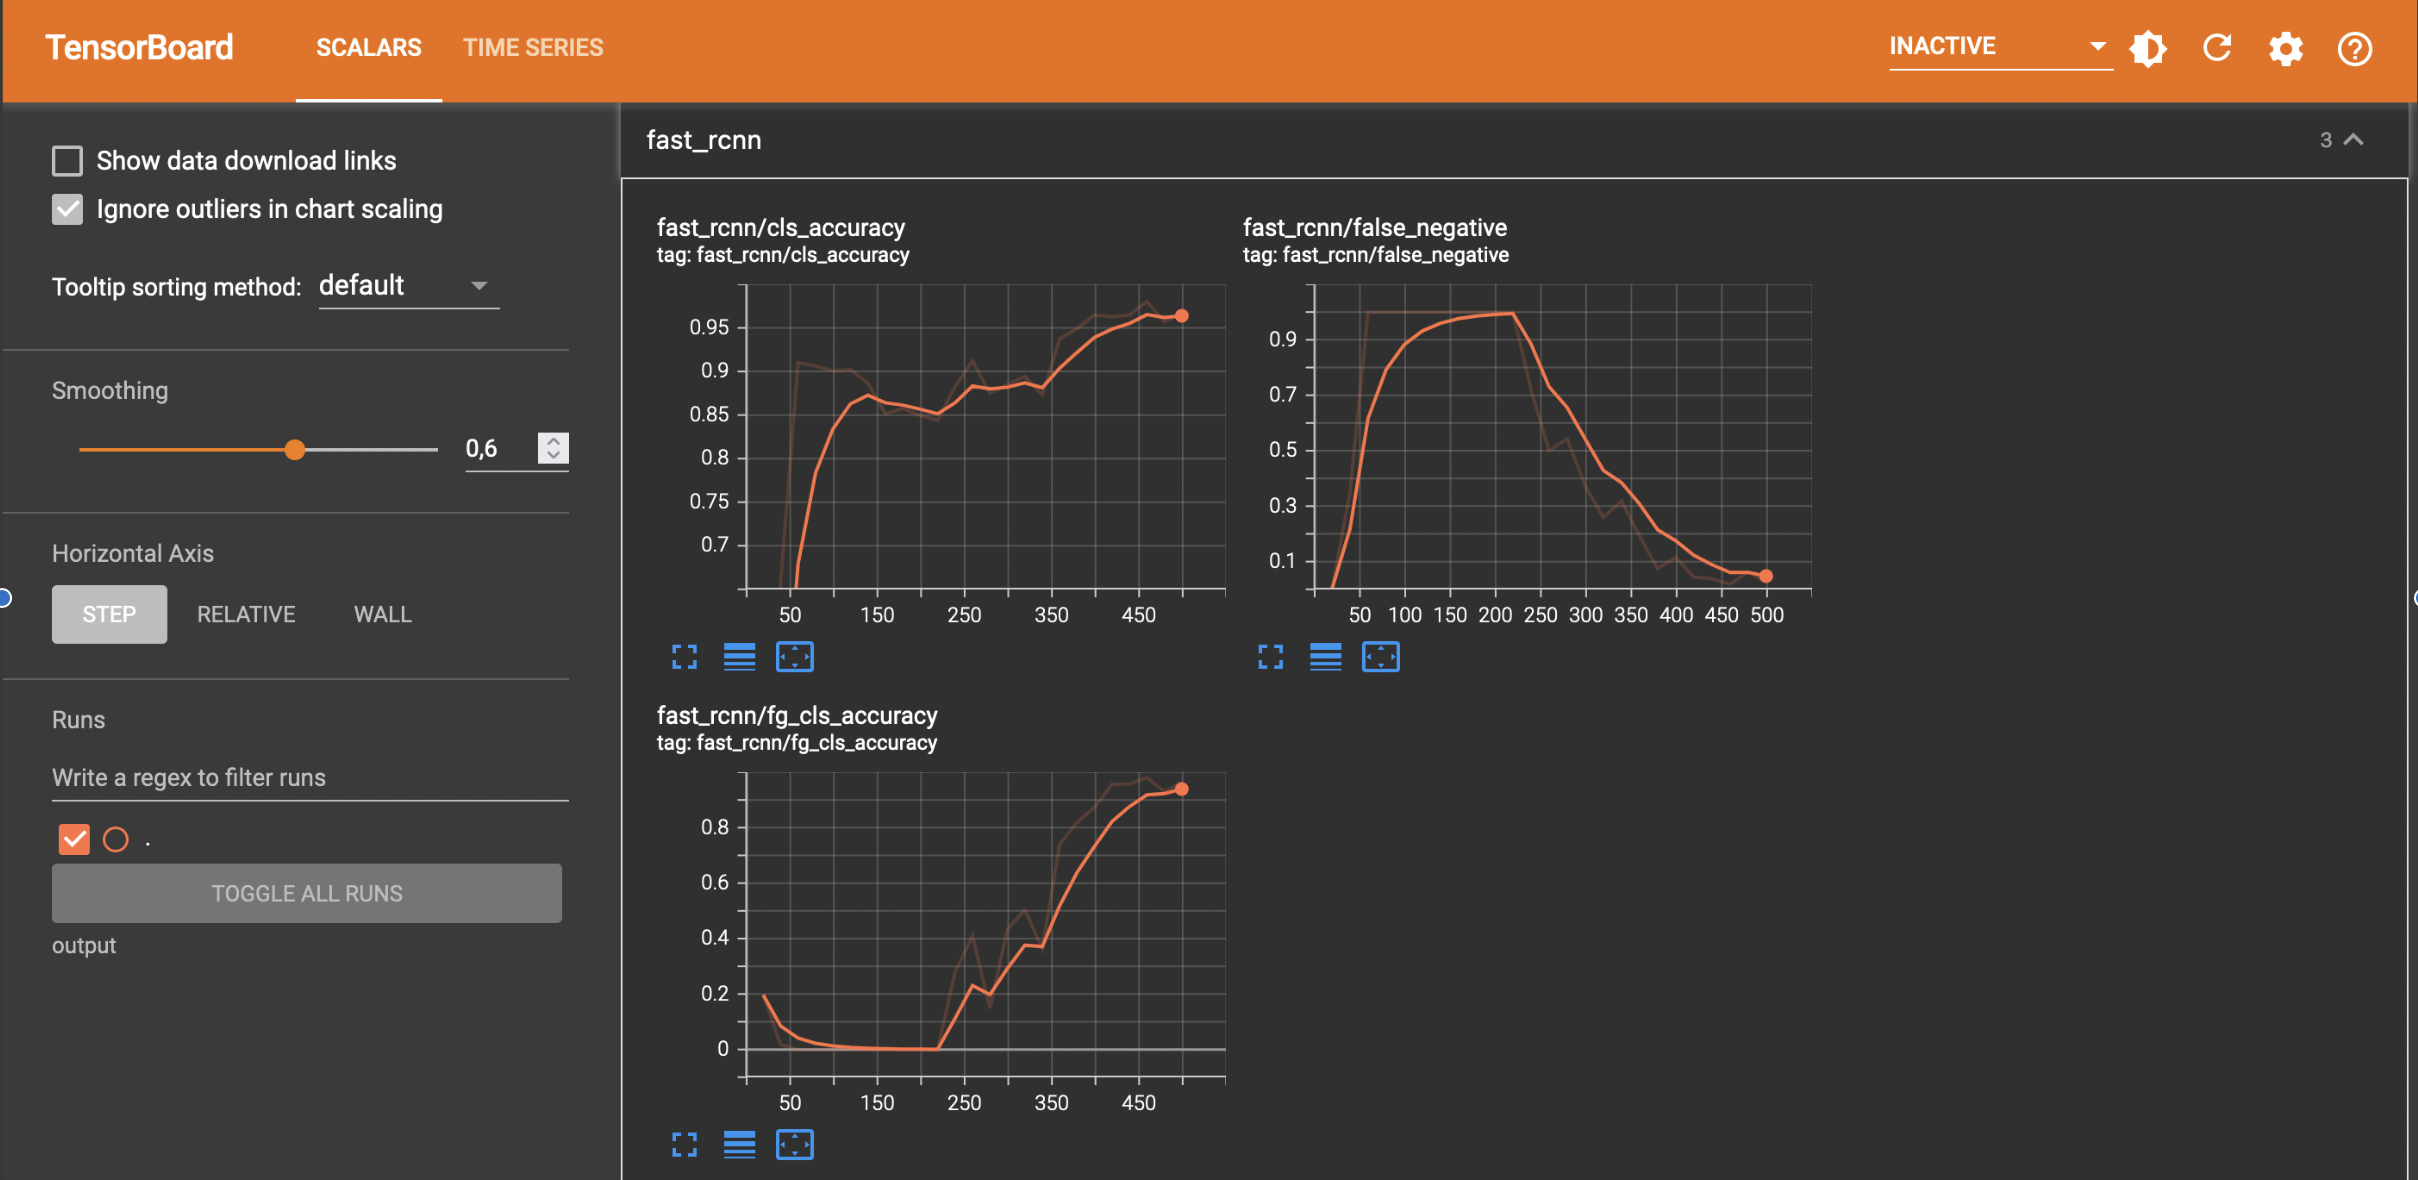
\includegraphics[width=\textwidth]{images/tensorboard_metric.png}
        \caption{Aperçu des métriques enregistrées dans TensorBoard}
        \label{fig:tensorboard_metric}
    \end{subfigure}
    % \scalebox{0.5}[0.5]{}
    % \caption{Aperçu du widget Tensorboard}
    % \label{fig:tensorboard_overview}
    % \scalebox{0.5}[0.5]{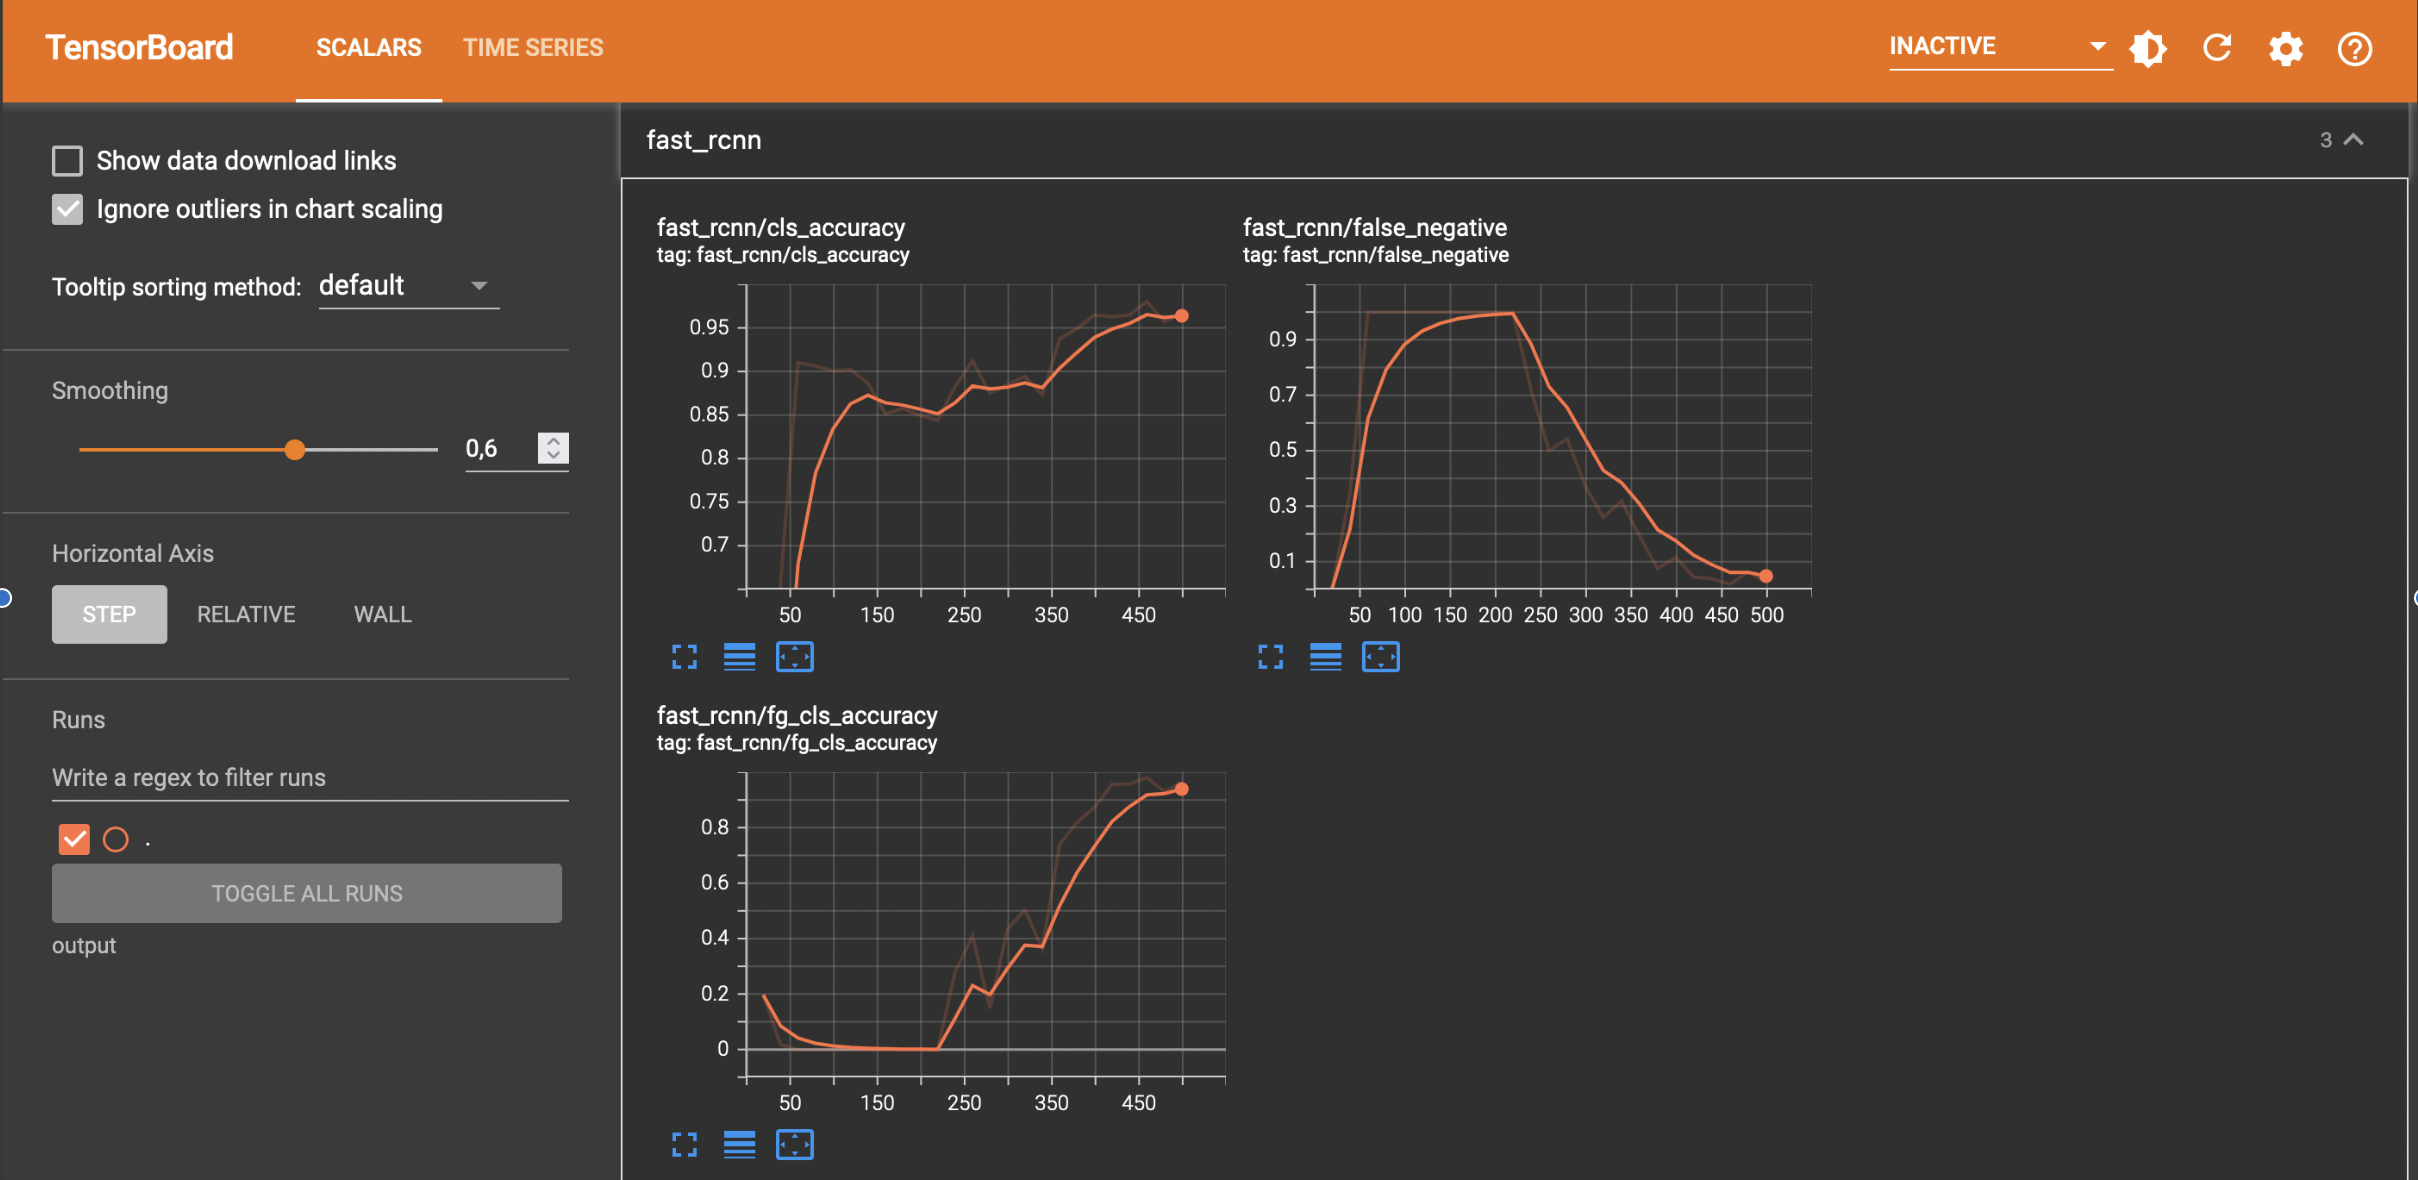
\includegraphics[width=\textwidth]{images/tensorboard_metric.png}}
    % \caption{Aperçu des métriques enregistrées dans TensorBoard}
    \caption{Aperçu de tensorboard et des métriques de faster RCNN}
\end{figure}
Detectron2 affiche aussi une loss total, nous n'avons pas réussis à déterminer la manière dont elle est calculée, mais elle reste un bon indicateur de la performance du model et de l'over/under fitting. De plus comme nous avons plusieurs modèles, nous pouvons les comparer entres eux puisques toutes erreurs sera identiques sur tous les modèles
\begin{figure}[hb!]
    \centering
    \scalebox{0.5}[0.5]{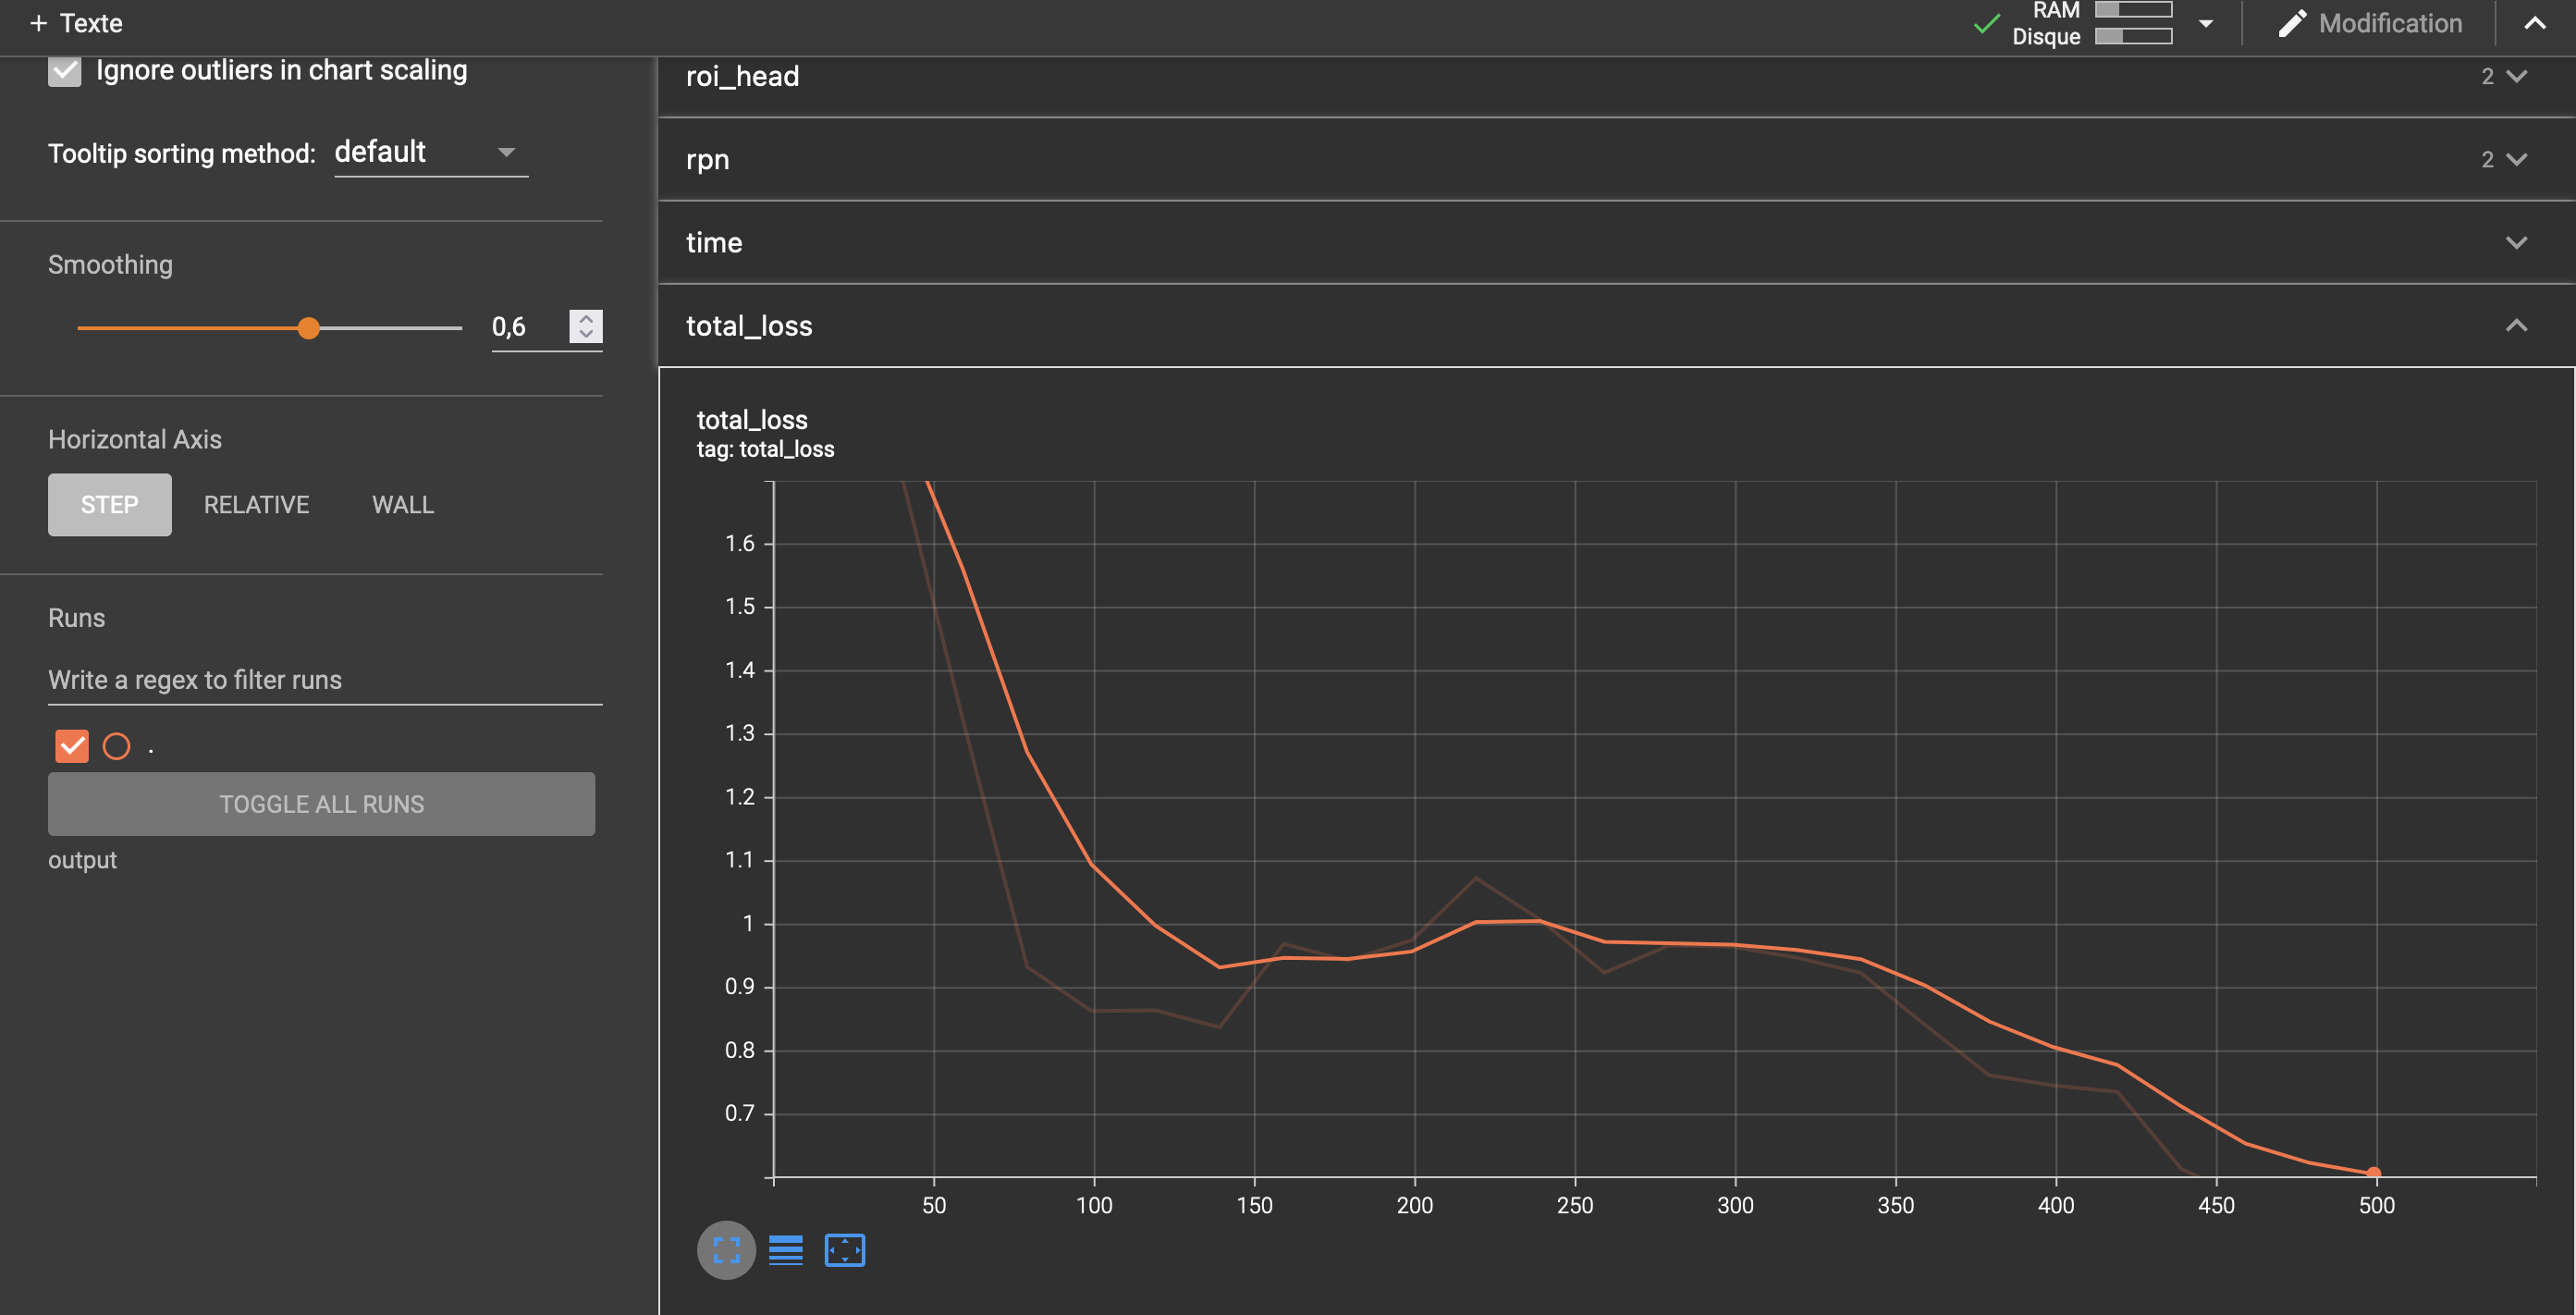
\includegraphics[width=\textwidth]{images/loss_faster_rcnn.png}}
    \caption{Aperçu de la loss total enregistrée dans TensorBoard}
    \label{fig:loss_faster_rcnn}
\end{figure}
Comme nous pouvons le voir dans la figure \ref{fig:loss_faster_rcnn}, nous n'avons ni d'overfit, ni d'underfit.


\section {Loss de RetinaNet}\label{anal:train_retina}
Dans cette section nous allons observer les métriques du modèle RetinaNet. Ce modèle enregistre moins de métriques, ceci est du au fait qu'il ne possède pas une architecture aussi complexe que Faster-RCNN. Alors que Faster-RCNN présentait des métriques pour certaines parties spécifiques du réseau, les RPN (Region Proposal Network) par exemple, RetinaNet ne présente que deux métriques relatives à l'entrainement : la loss de classification ainsi que la loss des bounding boxes.
\begin{figure}[h!]
    \begin{subfigure}[h]{0.49\textwidth}
        \centering
        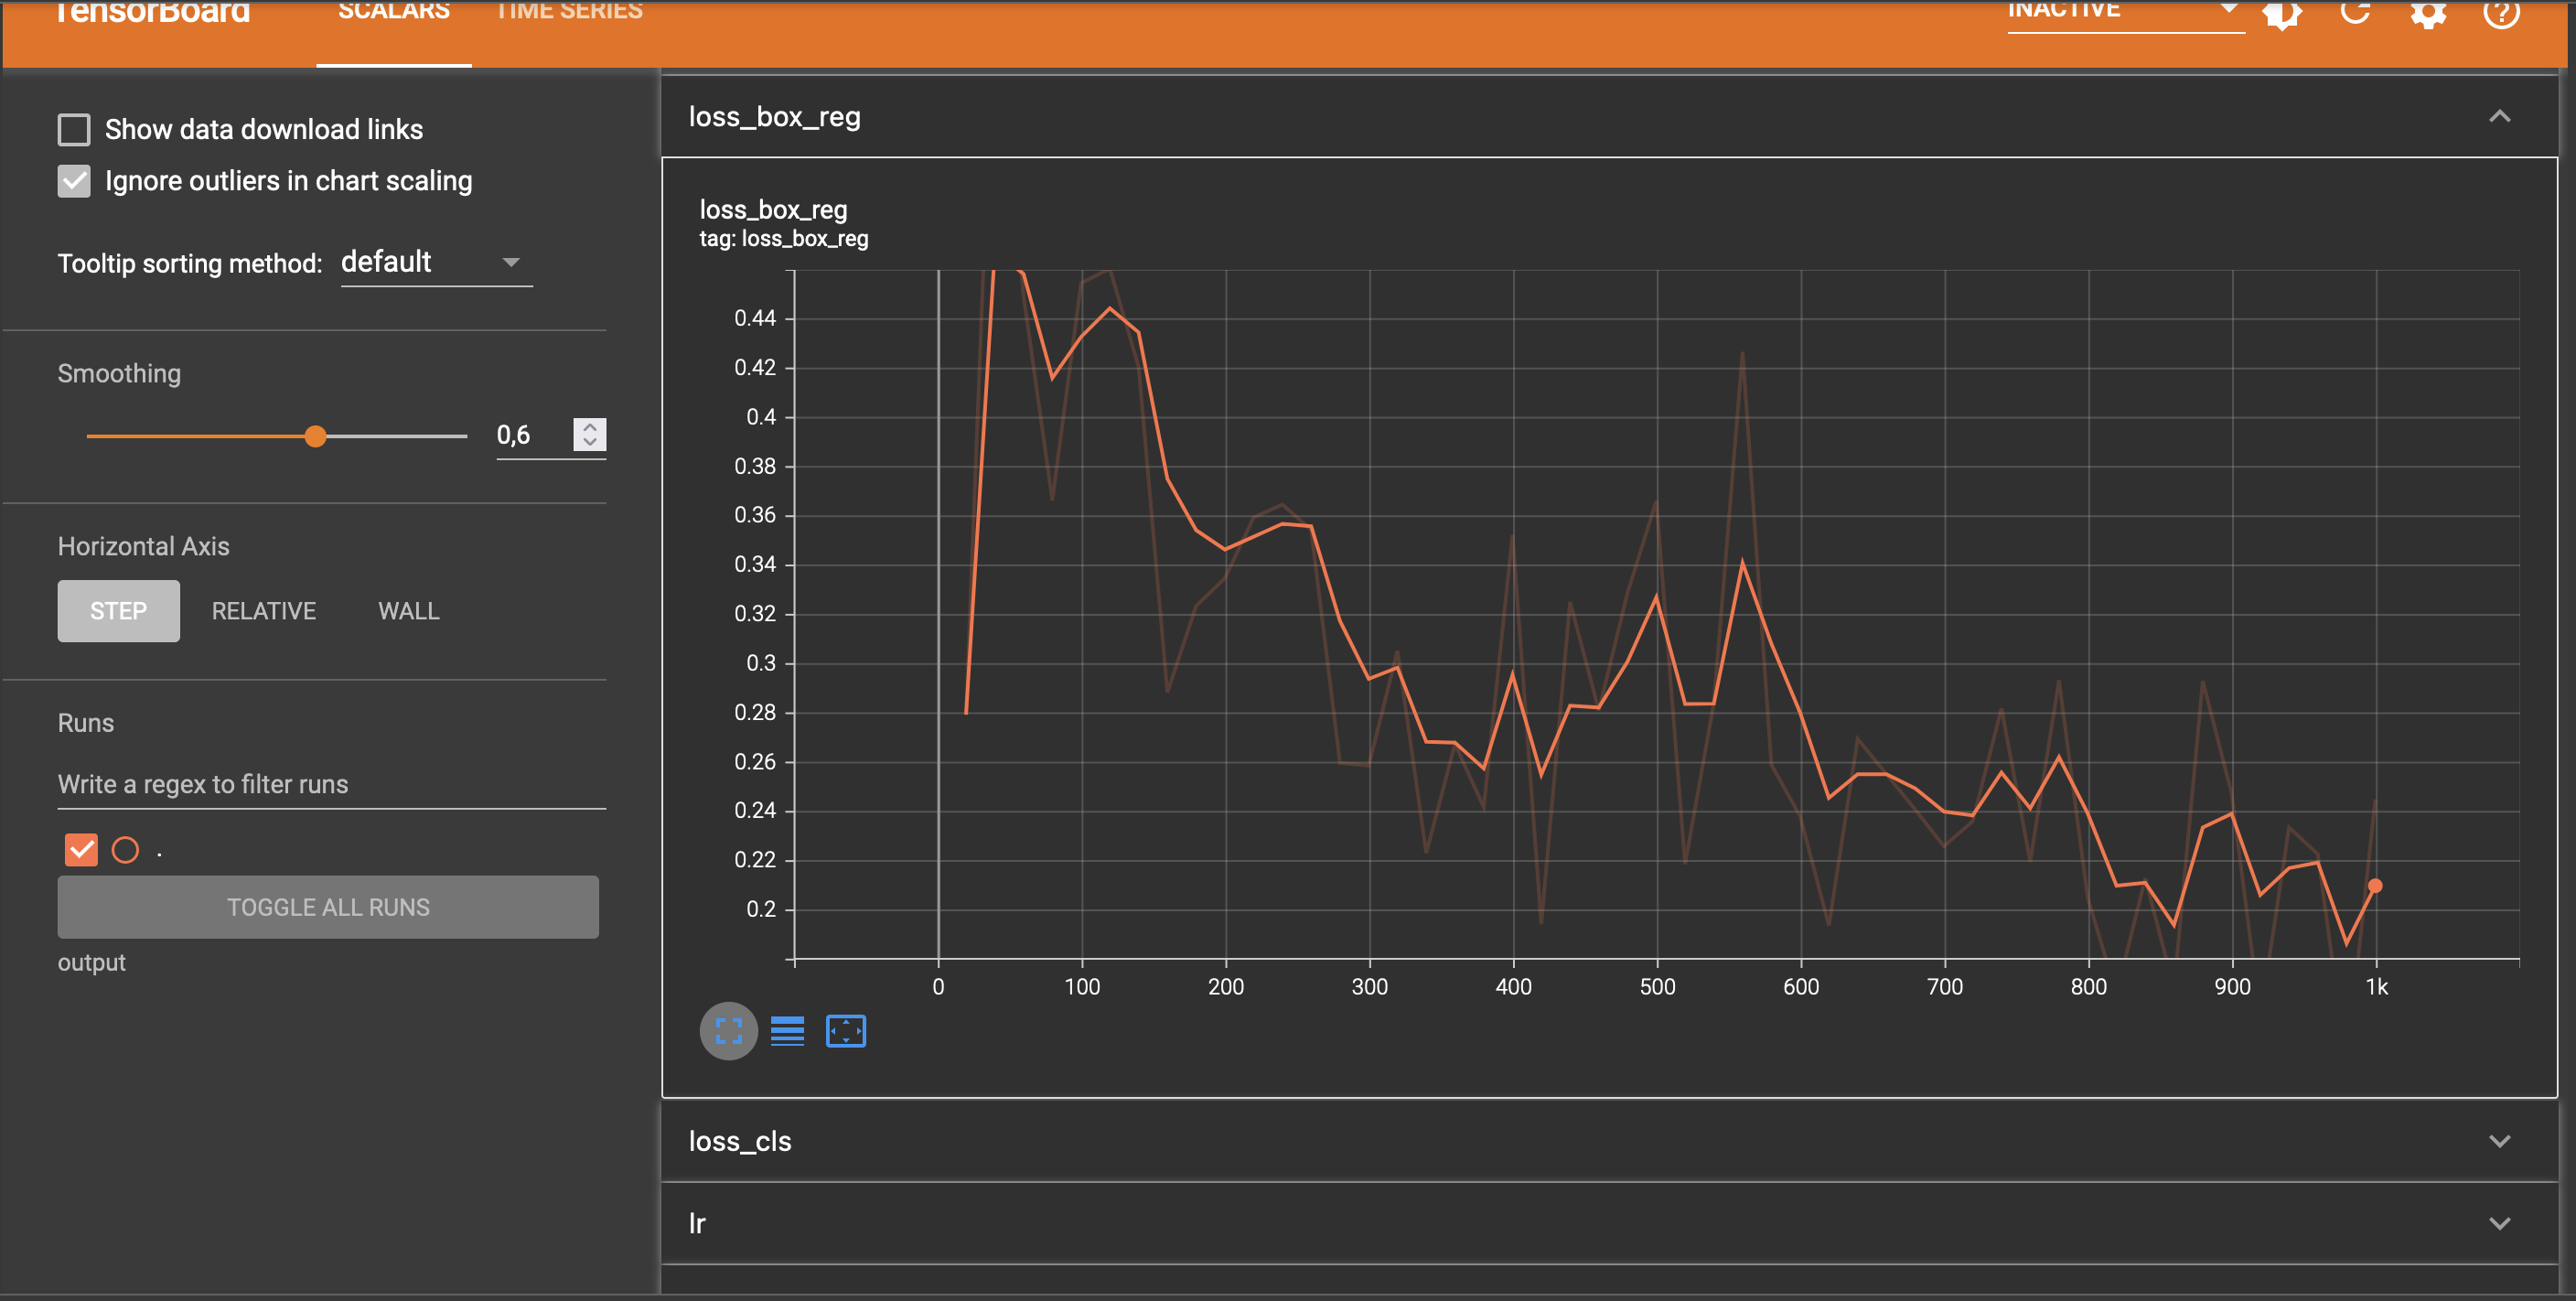
\includegraphics[width=\textwidth]{images/tensorboard_retina_net_loss_box.png}
        \caption{Loss des bounding boxes}
        \label{fig:loss_retinanet_box}
    \end{subfigure}
    \begin{subfigure}[h]{0.49\textwidth}
        \centering
        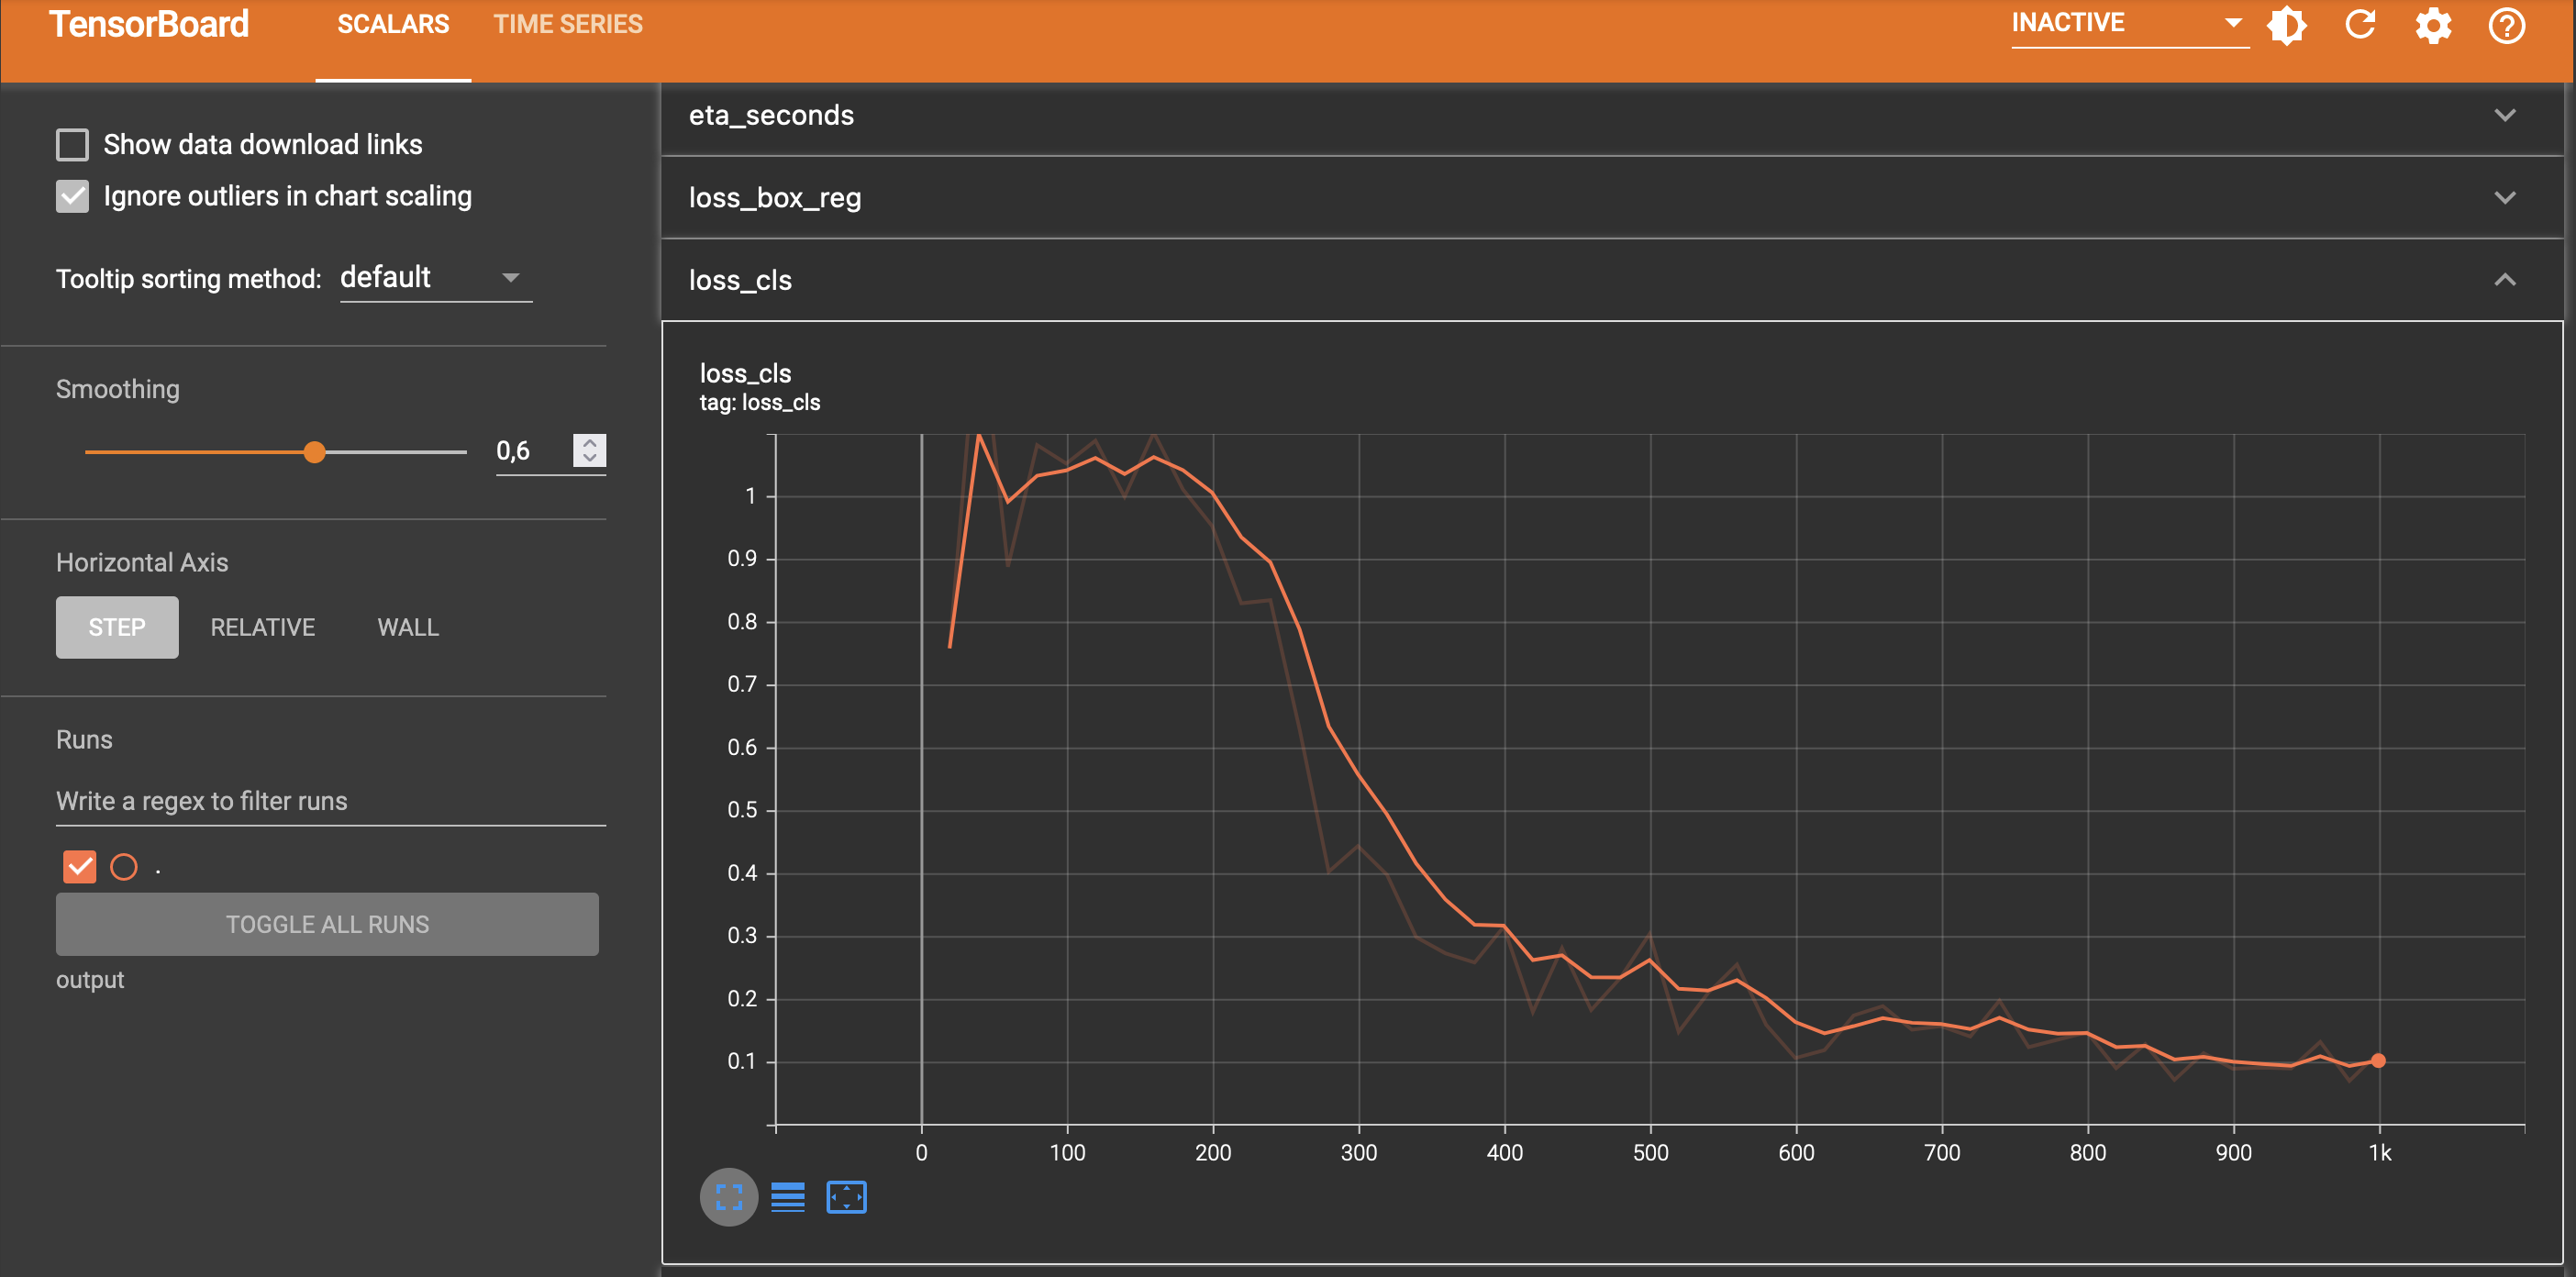
\includegraphics[width=\textwidth]{images/tensorboard_retina_net_loss_cls.png}
        \caption{Loss pour la classification}
        \label{fig:loss_retinanet_cls}
    \end{subfigure}
    \caption{Les métriques de RetinaNet durant un entrainement}
\end{figure}
Nous pouvons observer que RetinaNet doit être plus entrainé, 1000 itérations contre 500 pour Faster-RCNN. Il ne faut pas confondre itérations et époch. Une époch représente un passage sur l'entièreté du dataset, tandis qu'une iteration est un pas vers la recherche d'un minimum durant l'optimisation de l'erreur. Nous avons déterminé ces hyperparamètres grâce à tensorboard qui permet durant l'entrainment d'avoir un aperçu des métriques. Fait intéressant, RetinaNet est plus rapide à entrainer (environ 10 minutes de moins que Faster-RCNN) ceci est surement du à son architecture plus simple qui nécessite donc moins de calcule.

% -- Vic : 

\section{Évaluations des deux modèles sélectionnés}

Après avoir testé plusieurs approches comme mentionnées dans le chapitre \ref{chap:Modeles}, nous avons retenu deux modèles dont nous allons ici comparer les scores d'évaluation :

\begin{itemize}
    \item[-] Faster R-CNN avec Detectron2 et
    \item[-] Retinanet avec Detectron2.
\end{itemize}

Voici donc un tableau résumant les average precision (AP) scores de chaque catégorie suivant le treshold, ainsi 

Scores par classe : 

\begin{center}
   \begin{tabular}{ | l | l || c |}
     \hline
     modèle & catégorie & AP score \\ \hline
     \multirow{2}{*} {Faster R-CNN} & crapaud-grenouille & 42.03 \\ 
     & triton & 42.58   \\ \hline
     \multirow{2}{*} {Retinanet} & crapaud-grenouille & 49.40 \\
    & triton & 0.00 \\
     \hline
   \end{tabular}
 \end{center}

 Bien que le score pour la classe crapaud-grenouille soit plus élevé à l'aide du modèle Retinanet, le score pour la classe triton est de zéro. Rappelons que la tâche initiale de ce projet est de compter le nombre de triton/crapaud-grenouille qui utilisent les crapauduc ; ainsi, nous avons choisi l'algorithme Faster R-CNN comme modèle final pour cette tâche de classification.

\subsection{Modèle final choisi}

\paragraph{Entraînement}

Voici donc comment nous avons premièrement entraîné notre modèle Faster R-CNN, avec Detectron 2 : 

\lstset{language=Python}
\begin{lstlisting}
cfg = get_cfg()
cfg.merge_from_file(model_zoo.get_config_file("COCO-Detection/
faster_rcnn_X_101_32x8d_FPN_3x.yaml"))
cfg.DATASETS.TRAIN = ("triton_train",)
cfg.DATASETS.TEST = ()
cfg.DATALOADER.NUM_WORKERS = 2
cfg.MODEL.WEIGHTS = model_zoo.get_checkpoint_url("COCO-Detection/
faster_rcnn_X_101_32x8d_FPN_3x.yaml")  
cfg.SOLVER.IMS_PER_BATCH = 2 
cfg.SOLVER.BASE_LR = 0.00020 
cfg.SOLVER.MAX_ITER = 500 
cfg.SOLVER.STEPS = []   
cfg.MODEL.ROI_HEADS.BATCH_SIZE_PER_IMAGE = 128  
cfg.MODEL.ROI_HEADS.NUM_CLASSES = 4 
\end{lstlisting}


\paragraph{Test}

Et voici donc le modèle construit pour tester nos données d'évaluation : 

\lstset{language=Python}
\begin{lstlisting}
# on recuperation des poids du modele qu'on vient d'entrainer
cfg.MODEL.WEIGHTS = os.path.join(cfg.OUTPUT_DIR, "model_final.pth")  
# determination d'un treshold pour le test
cfg.MODEL.ROI_HEADS.SCORE_THRESH_TEST = 0.7  
# construction du predicteur
predictor = DefaultPredictor(cfg)
\end{lstlisting}

Le treshold choisi pour le test ci-dessus indique donc qu'on considérera une image comme étant prédite d'une certaine classe si le modèle est sûr à au moins 70\% de sa classification.\newline

Voici deux exemples de résultats de classification par notre modèle ainsi créé :

\begin{figure}[H]
    \centering
    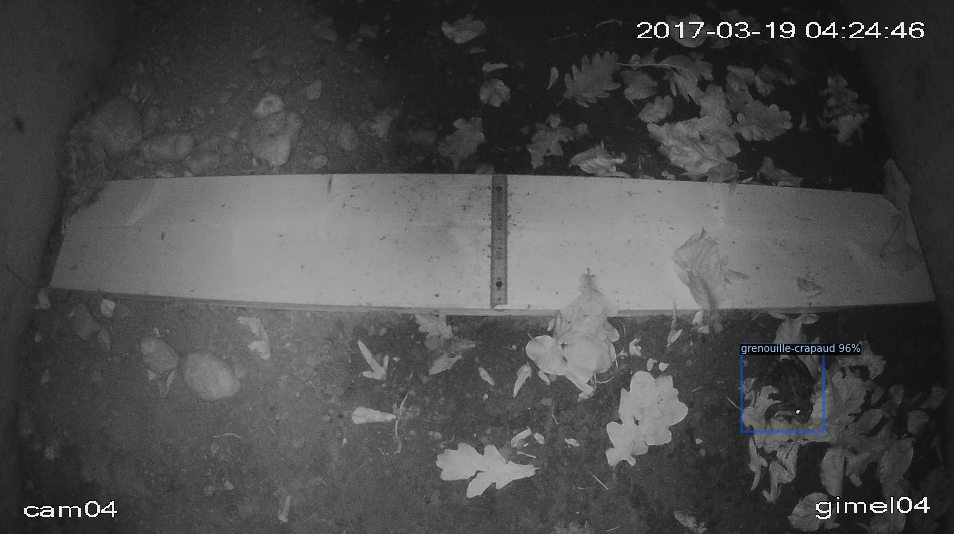
\includegraphics[width=300px]{images/Eval_FasterRCNN_crapGren.png}
    \caption{Prédiction de Faster R-CNN - crapaud-grenouille}
    \label{fig:fasterRcnn_crapGren}
\end{figure}

\begin{figure}[H]
    \centering
    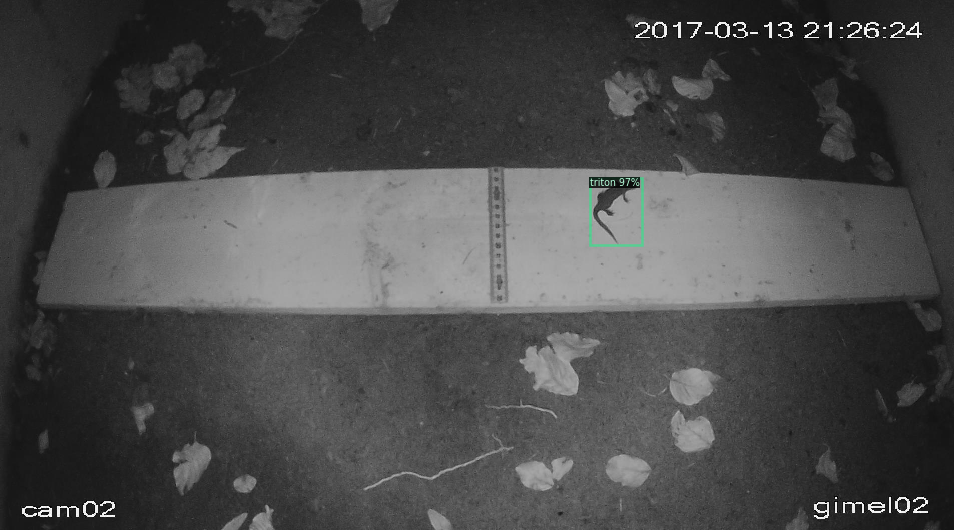
\includegraphics[width=300px]{images/Eval_FasterRCNN_triton.png}
    \caption{Prédiction de Faster R-CNN - triton}
    \label{fig:fasterRcnn_triton}
\end{figure}

Validation (résultats) important de dire que images sont similaires à celles deja vues blabla --> Joris (précision sur ce qui est dit..)

\section{Où est le problème}

Nous avons donc des résultats qui approchent ceux de l'état de l'art en 2019 selon \url{https://paperswithcode.com/sota/object-detection-on-coco}. Nous avons aussi des modèles qui sont correctement entrainés puisque, nous l'avons vu dans la partie \ref{anal:train_rcnn} ainsi que \ref{anal:train_retina}, les métriques indiquent qu'ils sont ni sous-entrainés ni sur-entrainés. Il nous faut donc observer des mauvaises classifications afin de comprendre les erreurs et de déterminer d'autres facteurs sur lesquels nous pouvons agir afin d'avoir de meilleurs résultats. En effet à l'heure où nous écrivons ces mots, un modèle basé sur DETR \footnote[1]{https://arxiv.org/pdf/2211.03594v1.pdf} atteint 64.5\% d'AP sur le benchmark COCO, ce qui est un score très élevé. Il existe donc des modèles SOTA bien meilleurs mais nous n'arrivons pas à les reproduire. Nous allons donc observer les erreurs de classification afin de comprendre ce qui ne va pas, mais avant nous aimerions faire remarquer qu'une explication possible est simplement la taille du Modèle. DETR, notre plus gros modèle, a 60 millions de paramètres alors que leur modèle en a 600 millions.
\subsection{Analyse des images non détectés par Faster-RCNN}
\begin{figure}[h]
    \centering
    \begin{subfigure}[h]{0.49\textwidth}
        \centering
        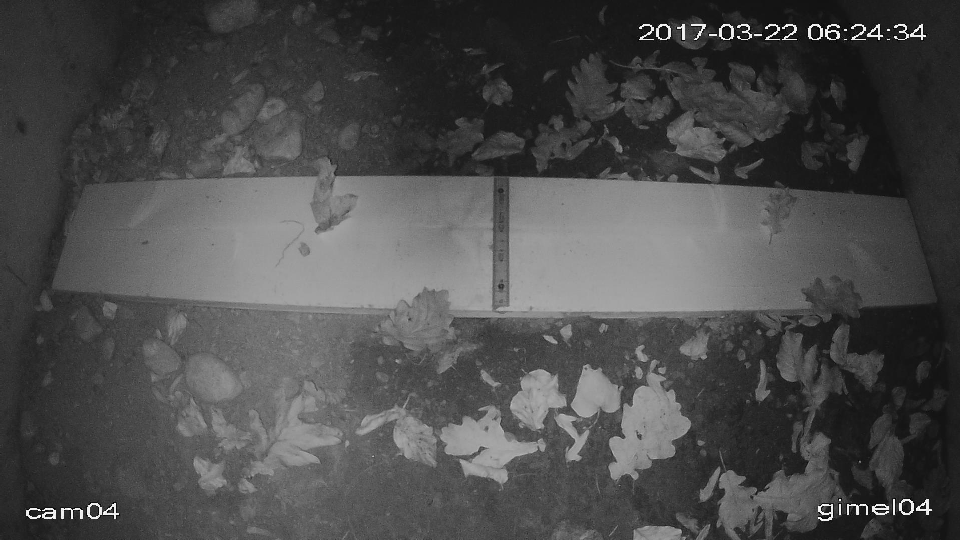
\includegraphics[width=0.9\textwidth]{images/failed_pred1_rcnn.png}
        \caption{Crapaud-grenouille caché}
        \label{fig:eval_fasterRCNN_a}
    \end{subfigure}
    \begin{subfigure}[h]{0.49\textwidth}
        \centering
        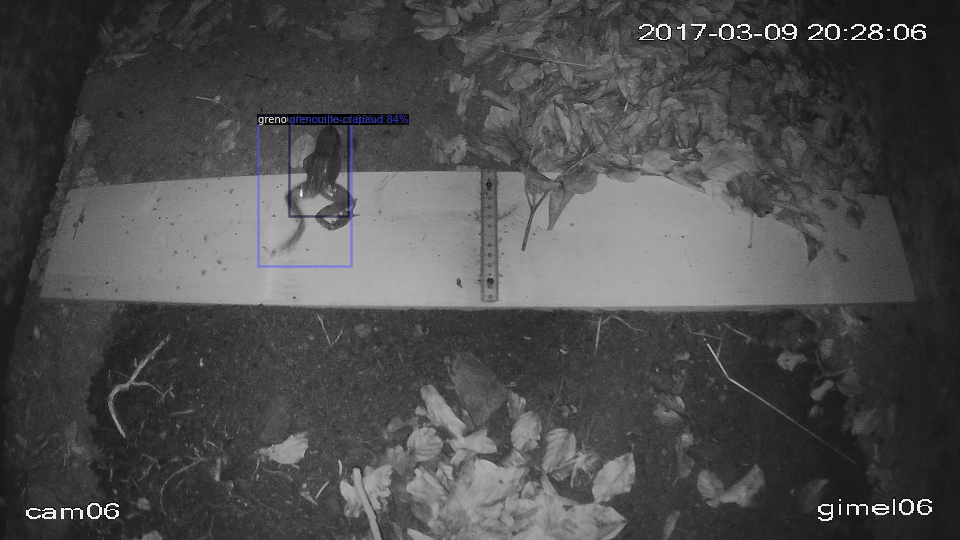
\includegraphics[width=0.9\textwidth]{images/failed_pred3_rcnn.png}
        \caption{Double bounding box}
        \label{fig:eval_fasterRCNN_b}
    \end{subfigure}
    \begin{subfigure}[h]{0.7\textwidth}
        \centering
        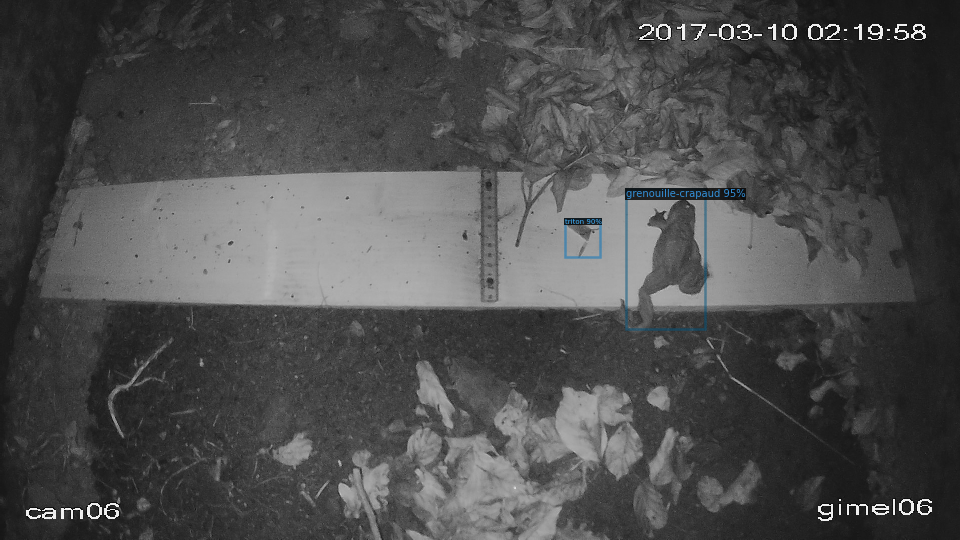
\includegraphics[width=0.9\linewidth]{images/failed_pred5_rcnn.png}
        \caption{Erreur de classification}
        \label{fig:eval_fasterRCNN_c}
    \end{subfigure}
    \caption{Exemple d'images mal prédites par Faster-RCNN}
    \label{fig:failed_pred_rcnn}
\end{figure}
La plupart des images qui présentent des erreurs pouvant expliquer le score de de Faster-RCNN ressemble aux images de la figure \ref{fig:failed_pred_rcnn}. 
Nous avons ici trois types d'erreurs. 
\paragraph{}
La première, qui est aussi une des plus fréquente, est la non détection d'animaux (souvent sur les bords de l'image). Le manque de luminosité ou la présence de feuille pourrait expliquer cela. Un pré-processing pourrait vérifier l'hypothèse de la luminosité. Cependant, nous ne pouvons pas vraiment faire de pré-processing pour la présence de feuille.
\paragraph{}
La seconde est aussi assez fréquente, il s'agit de la présence de multiples bounding box sur un même animal. Même si c'est étonnant, cette erreur ne devrait pas affecter les scores sur le benchmark. Nous avons aussi tuner le threeshold de confiance pour éviter ce genre d'erreur.
\paragraph{}
La dernière est la seul occurence de ce type observée sur le set de teste, on peut voir qu'un bout de feuille est mal classifié avec pourtant une accuracy de 90\%. Et ceci sans raisons visibles.
%  Nous pouvons nous demander si la planche à vraiment été bénéfique, en effet la plupart des annotations sont sur la planche, là où la planche permet rapidment d'apercevoir un animal. Le modèle a peut-être appris qu'il est plus probable de voir un animal donc peut-être plus habitué à voir des animaux à cet endroit.
En conclusion, Faster-RCNN est vraiment bon et les erreurs ne présentent pas de grâve erreur d'entrainement.

\subsection{Analyse des images non détectés par RetinaNet}
\begin{figure}[ht]
    \centering
    \begin{subfigure}[h]{0.49\textwidth}
        \centering
        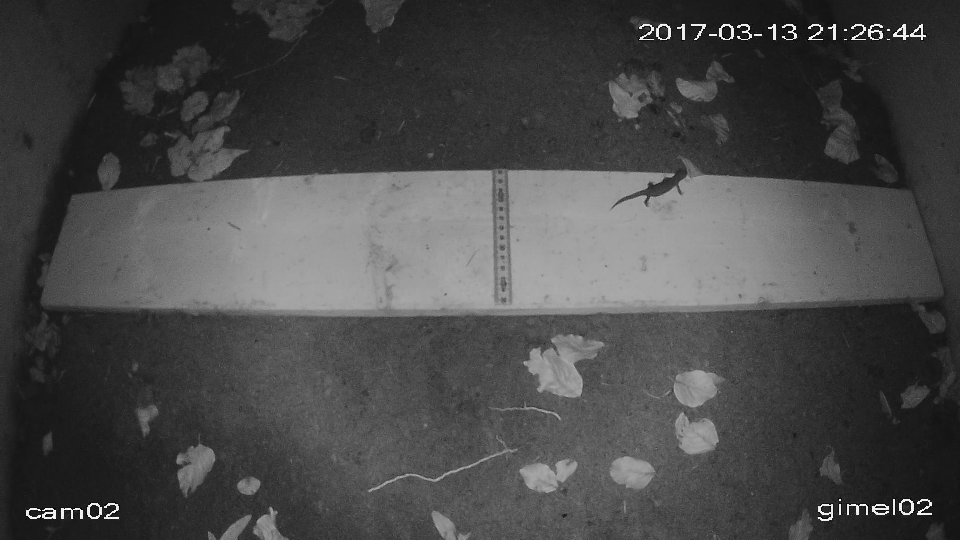
\includegraphics[width=0.9\textwidth]{images/failed_pred3_retina.png}
        \caption{Triton jamais détecté}
        \label{fig:eval_retina_a}
    \end{subfigure}
    \begin{subfigure}[h]{0.49\textwidth}
        \centering
        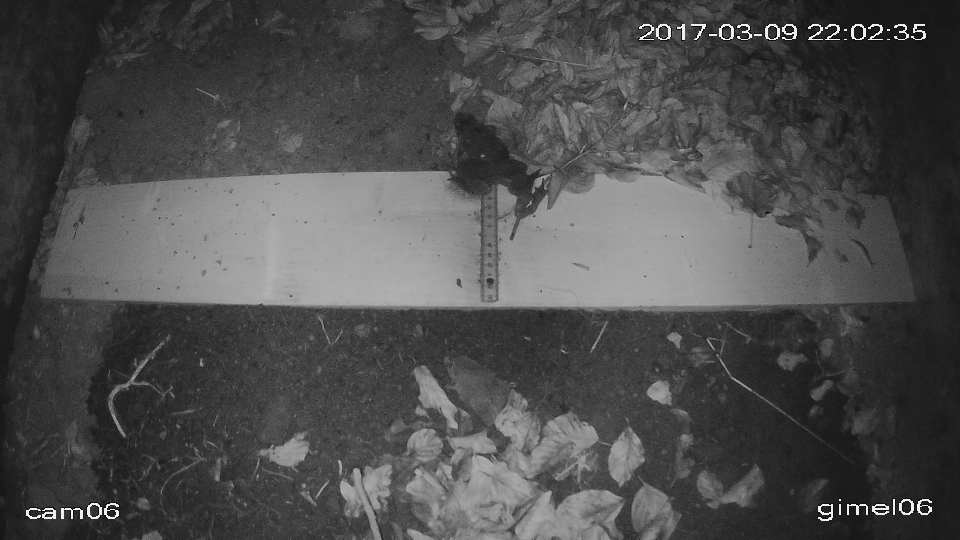
\includegraphics[width=0.9\textwidth]{images/failed_pred5_retina_big.png}
        \caption{Non détection du crapaud}
        \label{fig:eval_retina_b}
    \end{subfigure}
    \begin{subfigure}[h]{0.7\textwidth}
        \centering
        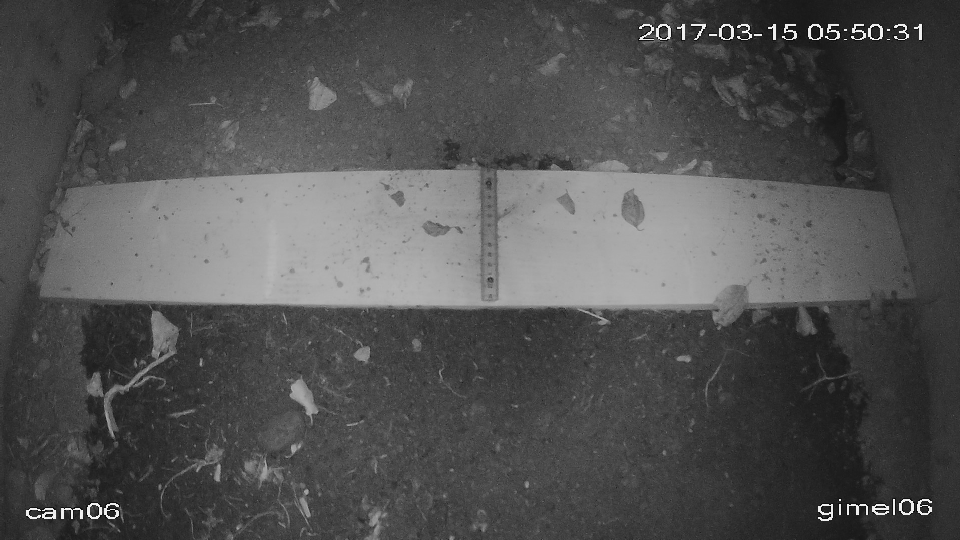
\includegraphics[width=0.9\linewidth]{images/failed_pred4_retina.png}
        \caption{Animal non détecté}
        \label{fig:eval_retina_c}
    \end{subfigure}
    \caption{Exemple d'images mal prédites par RetinaNet}
    \label{fig:failed_pred_retina}
\end{figure}
Nous pouvons voir dans la figure \ref{fig:failed_pred_retina} que RetinaNet ne detecte jamais les tritons. Nous avons pensé que c'était du à la petite taile de ces derniers, cependant nous pouvons observé que l'image \ref{fig:eval_retina_b} est un gros crapaud qui n'est pas non plus reconnu. Il faut remarquer que du set de test, il s'agit de l'unique occurence d'une telle erreur.
On peut noter que les crapauds-grenouilles sont toujours très bien detecté. L'image \ref{fig:eval_retina_c} nous montre un problème similaire à celui vu prédécement sur l'image \ref{fig:eval_fasterRCNN_a} ce qui tend à confirmer l'hypothèse du manque de lumière sur les cotés.
\paragraph{Conclusion}. Nos deux modèles semblent avoir des difficultés avec les animaux qui passent par les cotés, il se peut, au vu des nombreuses annotations d'entrainement bien centrées, que les modèles aillent appriez à détecter les animaux au centre de l'image. Néanmoins, un ajustement de la luminosité serait une piste de réflexion.